\documentclass{boi2014-se}

\usepackage{enumitem}
\usepackage{todonotes}
\usepackage{wrapfig}

\renewcommand{\DayNum}{2}
\renewcommand{\TaskCode}{demarcation}
\renewcommand{\TaskName}{Landuppdelning}
\renewcommand{\TaskVersion}{1.2}

\newcommand{\constant}[1]{{\tt #1}}

\begin{document}
    \begin{wrapfigure}{r}{3cm}
        \vspace{-24pt}
		\includegraphics[width=3cm]{\TaskCode.jpeg}
	\end{wrapfigure}

    Ön Bitopia styrdes länge av den rättvise kung Bytasar.
    Efter hans plötsliga död kunde dock inte hans två söner,
    tvillingarna Biteon och Byteon, enas om vem som skulle bli hans efterträdare.
    De bestämde sig därför för att dela upp ön i två provinser, och
    härska över dem oberoende av varandra.

    På en rektangulär karta kan Bitopia ses som en polygon bestående av $N$ hörn.
    Varje sida av polygonen är parallell till en sida av kartan, och
    två på varandra följande sidor är alltid vinkelräta mot varandra.
    Ingen sida av polygonen korsar eller vidrör någon annan sida, förutom
    de gemensamma ändpunkterna för efterföljande sidor.

    Biteon och Byteon vill, med hjälp av ett linjesegment, dela upp polygonen i
    två kongruenta delar. (Två figurer är kongruenta om den ena kan transformeras till
    den andra genom en kombination av reflektioner, rotationer och translationer.)
    Linjesegmentet ska ligga inuti polygonen och vara
    parallellt med någon av kartans sidor. Koordinaterna för polygonens hörn är heltal och
    detsamma måste även gälla för linjesegmentets ändpunkter.
 
    Biteon och Byteon har bett dig kolla om en sådan uppdelning är möjlig.
 
    \Task

    Givet formen på ön, avgör om den kan delas upp i två kongruenta delar
    med hjälp av ett horisontellt eller vertikalt linjesegment. Om det är
    möjligt, hitta ett sådant segment.

    \Input
    Första raden i indata består av ett enda heltal $N$, antal hörn i polygonen.
    Den $i$:te av de följande $N$ raderna innehåller två mellanslagsseparerade heltal
    $X_i$ och $Y_i$ ($0 \le X_i, Y_i \le 10^9$), koordinaterna för polygonens $i$:te hörn.

    \Output
    Ditt program ska skriva ut en enda rad. Om det är möjligt att dela upp ön i
    två kongruenta delar med hjälp av ett horisontellt eller vertikalt linjesegment,
    så ska ett sådant segment ges. Detta görs genom att skriva ut de $4$ heltalen 
    $x_1$, $y_1$, $x_2$ och $y_2$, där $(x_1, y_1)$ och $(x_2, y_2)$ är koordinaterna
    för linjesegmentets ändpunkter. Det måste gälla att $x_1 = x_2$ eller $y_1 = y_2$.

    Om ingen sådan uppdelning är möjlig så ska ordet \constant{NO}
    skrivas ut.

    \clearpage

    \Examples
	\example
	{
		10  \newline
		0 0 \newline
		1 0 \newline
		1 1 \newline
		3 1 \newline
		3 5 \newline
		2 5 \newline
		2 3 \newline
		1 3 \newline
		1 2 \newline
		0 2
	}
	{
		1 2 3 2
	}
	{
        Notera att {\tt 3 2 1 2} också är en giltig lösning.

        \begin{center}
            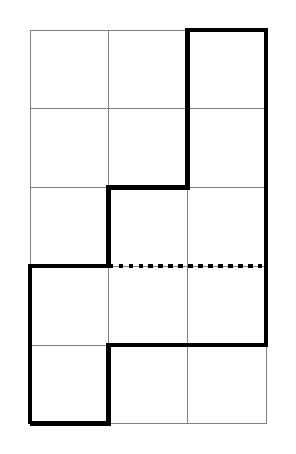
\begin{tikzpicture}
            \draw[help lines] (0,0) grid (3,5);
            \draw[ultra thick] (0,0) -- (1,0) -- (1,1) -- (3,1) -- (3,5) --
                         (2,5) -- (2,3) -- (1,3) -- (1,2) -- (0,2) -- (0,0);
            \draw[ultra thick,dotted] (1,2) -- (3,2);
            \end{tikzpicture}
        \end{center}
	}

	\example
	{
		6 \newline
		0 0 \newline
		1 0 \newline
		1 1 \newline
		2 1 \newline
		2 2 \newline
		0 2
	}
	{
		NO
    }
    {
        I det här fallet finns det inget sätt att dela ön i två kongruenta
        delar.
        \begin{center}
            
\begin{tikzpicture}
            \draw[help lines] (0,0) grid (2,2);
            \draw[ultra thick] (0,0) -- (1,0) -- (1,1) --
                         (2,1) -- (2,2) -- (0,2) -- (0,0);
            \end{tikzpicture}
        \end{center}
	}

    \Scoring

    \begin{description}
        \item[Deluppgift 1 (12 poäng).] $4 \le N \le 100\ 000$.
        Varje horisontell eller vertikal linje som delar polygonen delar den i
        exakt två delar.
        
        \item[Deluppgift 2 (15 poäng).] $4 \le N \le 200$.
        \item[Deluppgift 3 (23 poäng).] $4 \le N \le 2\ 000$.
        \item[Deluppgift 4 (50 poäng).] $4 \le N \le 100\ 000$.
    \end{description}

    \Constraints

    \begin{description}
        \item[Tidsgräns:] 0.5 s.
        \item[Minnesgräns:] 256 MB.
    \end{description}

\end{document}
